\documentclass[11pt, a4paper, oneside]{article}

\usepackage[T1]{fontenc}
%\usepackage[utf8]{inputenc}
%\usepackage[english, polish]{babel}
\usepackage{polski}
\usepackage{setspace}
\usepackage{indentfirst}

\usepackage[left=2.0cm, right=2.0cm, top=1.5cm, bottom=2cm]{geometry}

\usepackage{fancyhdr}
\usepackage[table]{xcolor}
\usepackage{graphicx}
\usepackage{amsmath}
\usepackage{amsthm,thmtools}
\usepackage[nottoc]{tocbibind}
\usepackage{ragged2e}
\usepackage{bbding}
\usepackage{makeidx}
\usepackage{titlesec}
\usepackage{tcolorbox}
\usepackage{url}
\usepackage{color}
\usepackage{setspace}
\usepackage[font=small,format=plain,labelfont=bf,up,textfont=it,up]{caption}
\usepackage{BeamerColor}
\usepackage{listings}
\usepackage{multirow}
\usepackage{changepage}
\usepackage{float}

\definecolor{mycolor1}{RGB}{0,0,128}
\definecolor{lightgray}{gray}{0.9}
\definecolor{lightlightgray}{gray}{0.95}
\definecolor{lightyellow}{RGB}{255,255,224}
\definecolor{lemonchiffon}{RGB}{255,250,205}

\definecolor{syntax}{RGB}{127,0,85}
\definecolor{comments}{RGB}{63,127,95}
\definecolor{strings}{RGB}{42,0,255}

\usepackage{mathtools}
\usepackage{siunitx}
\usepackage{cases}
\usepackage{lmodern}
%\usepackage{floatrow}
\usepackage{bm}
\newcommand{\matr}[1]{\mathbf{#1}}
\newcommand{\vect}[1]{\bm{\mathbf{#1}}}
\newcommand{\integrand}[1]{\left(#1\right)}
\DeclareRobustCommand*{\drv}{\mathop{}\!\mathrm{d}}
\DeclareRobustCommand*{\intdt}{\mathop{}\!\mathrm{dt}}

\renewcommand*\lstlistingname{Kod źródłowy}

\lstdefinestyle{mycpp} {
    language=C, % choose the language of the code
    alsolanguage=C++,
    basicstyle=\linespread{0.9}\fontfamily{lmtt}\selectfont\small\color{black},
    keywordstyle={\bfseries\color{syntax}}, % style for keywords
    emph={int,char,double,float,unsigned,printf,getchar,putchar,
sprintf,scanf,fopen,fscanf,fprintf,fclose,pthread_self,pthread_create,sleep,exit,pthread_t,
pthread_exit,pthread_cancel,pthread_join,pthread_attr_init,pthread_attr_setdetachstate,pthread_attr_destroy,
pthread_attr_getdetachstate,pthread_attr_setdetachstate,pthread_attr_getinheritsched,pthread_attr_setinheritsched,
pthread_attr_getschedpolicy,pthread_attr_setschedpolicy,pthread_attr_getschedparam,pthread_attr_setschedparam,
pthread_attr_getscope,pthread_attr_setscope,pthread_attr_getstacksize,pthread_attr_getstackaddr,pthread_attr_setstacksize,
pthread_attr_setstackaddr,pthread_attr_t,srand,time,rand,pthread_mutex_init,pthread_mutex_t,pthread_mutex_destroy,
pthread_mutex_lock,pthread_mutex_timedlock,time_t,pthread_mutex_trylock,pthread_mutex_unlock,
pthread_cond_init,pthread_cond_destroy,pthread_cond_wait,pthread_cond_timedwait,pthread_cond_signal,pthread_cond_broadcast,
pthread_barrier_init, pthread_barrier_t,pthread_barrierattr_t,pthread_barrier_wait,pthread_barrier_destroy,
pthread_cond_t,pthread_mutexattr_t,pthread_condattr_t,ChannelCreate,ChannelCreate_r,
ChannelDestroy,ChannelDestroy_r,ChannelAttach,ChannelDetach,MsgReceive,MsgReply,MsgSend,strerror,ConnectAttach,ConnectAttach_r,
pid_t,uint32_t,ConnectDetach,ConnectDetach_r,MsgSend_r,MsgReceive_r,name_attach,name_detach,name_open,name_close,
open,MsgReply_r,atoi,strcpy,_uint16,_int8,_uint8,_int32,MsgSendPulse,MsgReceivePulse,clock_gettime,perror,
clock_getres,clock_settime,ctime,nanosleep,delay,select,alarm,nanospin,timer_create,timer_settime,timer_gettime,timer_delete,
getpid},
    emphstyle={\bfseries\color{syntax}},
    stringstyle=\color{strings},
    commentstyle={\fontfamily{lmtt}\selectfont\color{comments}},
    numbers=left, % where to put the line-numbers
    numberstyle=\tiny, % the size of the fonts that are used for the line-numbers
    %backgroundcolor=\color{lemonchiffon},
    backgroundcolor=\color{lightgray},
    showspaces=false, % show spaces adding particular underscores
    showstringspaces=false, % underline spaces within strings
    showtabs=false, % show tabs within strings adding particular underscores
    frame=single, % adds a frame around the code
    tabsize=2, % sets default tabsize to 2 spaces
    rulesepcolor=\color{gray},
    rulecolor=\color{black},
    captionpos=t, % sets the caption-position to bottom
    breaklines=true, % sets automatic line breaking
    breakatwhitespace=false,
    xleftmargin=20pt,
    xrightmargin=20pt,
    aboveskip=12pt,
    belowskip=12pt,
    escapeinside={(*@}{@*)},
%   frameround=tttt,
   framexleftmargin=5mm,
   frame=shadowbox,
   rulesepcolor=\color{lightgray},
   extendedchars=\true,
   inputencoding=utf8,
}

\begin{document}
\hspace*{-\parindent}%
\begin{minipage}{\textwidth}
  \begin{minipage}{.7\textwidth}
   \begin{flushleft}
	Programowanie Równoległe i Rozproszone - sem. zimowy 2020/2021
	\end{flushleft}
  \end{minipage}
  \begin{minipage}{.3\textwidth}
    \begin{flushright}
	Agnieszka Jurkiewicz \\
	Maciej Pikuliński \\
	Tomasz Szczepański
	\end{flushright}
  \end{minipage}%
\end{minipage}
\begin{center}
{\Large \textbf{Optymalizacja: Metoda optymalizacji rojem cząstek (PSO) i poszukiwań losowych (Monte Carlo)}}
\end{center}

\section{Wstęp teoretyczny}
 
W ramach projektu zrealizowano wersję sekwencyjną i równoległą (OpenMP) algorytmów optymalizacji rojem cząstek (PSO) i poszukiwań losowych (Monte Carlo). Implementację przetestowano rozwiązując dwa zadania optymalizacji, w tym - standardową funkcję testową algorytmów optymalizacyjnych - funkcję Rosenbrocka. Sprawozdanie rozpoczyna się krótkim wstępem teoretycznym wraz z uwagami dotyczącymi specyficznych rozwiązań naszej implementacji. Dalej, przedstawiono najważniejsze elementy wersji równoległych algorytmów. Kolejna część sprawozdania prezentuje wykonane testy numeryczne i płynące z nich wnioski.

\subsection{Algorytm optymalizacji cząstek (PSO)} 

Algorytm optymalizacji cząstek (PSO, ang. {\it Particle Swarm Optimization}) został zainspirowany stadnym zachowanie zwierząt, np. ławic ryb czy kluczy ptaków. Na kierunek ruchu pojedynczego osobnika -- cząstki -- wpływa ruch pozostałych osobników w stadzie -- populacji. Przyjmijmy, że stado szuka współrzędnej $\vect{x} \in \mathcal{D}^{n}$, dla której funkcja celu $f\left(\vect{x}\right)$ przyjmuje minimalną wartość. Matematycznie, zachowanie $j$-tej cząstki w $k$-elementowej populacji możemy zapisać następująco
\begin{equation}
\begin{cases}
\vect{v}_{i + 1, j} = \omega \vect{v}_{i, j} + c_{1} \epsilon_{1} \left(\vect{p}_{i, j} - \vect{x}_{i, j}\right) + c_{2} \epsilon_{2} \left(\vect{q}_{i} - \vect{x}_{i, j}\right) \\
\vect{x}_{i + 1, j} = \vect{x}_{i, j} + \vect{v}_{i + 1, j},
\end{cases}
\end{equation}
gdzie $\vect{x}_{i, j}$ i $\vect{v}_{i, j}$ to odpowiednio wektory położenia i prędkości w generacji $i$, zmienne skalarne $\omega$, $c_1$, $c_2$ to wagi, a $\epsilon_{1}$ i  $\epsilon_{2}$ to pewne zmienne losowe. Najbardziej istotną rolę odgrywają jednak wektory $\vect{p}_{i, j}, \ \vect{q}_{i} \in \mathcal{R}^{n}$ odpowiedzialne za inteligencję roju. Wektor $\vect{q}_{i}$ reprezentuje położenie o najmniejszej znalezionej dotychczas funkcji celu w całej populacji, a analogiczny wektor $\vect{p}_{i, j}$ ogranicza swoją pamięć jedynie do danej, $j$-tej cząstki - oznacza dotychczasowe najlepsze ze względu na wartość funkcji celu położenie cząstki.

Zmienne losowe $\epsilon_{1}$ i $\epsilon_{2}$ odzwierciedlają biologiczną genezę modelu. Przyjmują wartości z zakresu $\epsilon_{i}, \epsilon{j} \in \left[0, \ 1\right]$ i w poszczególnych generacjach decydują w jakim stopniu trajektoria danej cząstki zostanie skierowana ku położeniom $\vect{p}_{i, j}, \ \vect{q}_{i}$. W przyjętym przez nas modelu zmienne losowe mają rozkład jednostajny. Warto także wspomnieć, że waga $\omega$ nazywana jest w literaturze \cite{BrattonKennedy} inercją, co~pomaga zinterpretować jej wpływ na ruch cząstki. Należy uważać na dobór jej wartości - zbyt duża wartość może prowadzić do niestabilności rozwiązań.

Dostępne są różne propozycje doboru wag modelu. Zachowanie roju zależy jednak także od kształtu funkcji celu i uniwersalne zestawy wag na ogół nie będą optymalne do rozwiązania dowolnego problemu. W związku z tym niezbędne może się okazać modyfikowanie ich wartości dla poszczególnych zadań optymalizacji. W przedstawionych w tym sprawozdaniu testach jako wartości wyjściowe wag przyjęto wartości zaproponowane w \cite{BrattonKennedy} i wynikające z tzw. \quotedblbase constriction method\textquotedblright.

Przestrzeń poszukiwań $\mathcal{D}^{n}$ może być ograniczona - w zaproponowanych w projekcie zadaniach mamy do czynienia z ograniczeniami kostkowymi. W przypadku tak postawionej optymalizacji z ograniczeniami powstaje pytanie co zrobić, jeżeli nowa pozycja cząsteczki, po losowaniu prędkości, znajduje się poza ograniczonym obszarem. Najprostszym rozwiązaniem wydaje się losowanie nowego położenia cząsteczki (nowej prędkości) aż będzie ono spełniało zadane ograniczenie. Takie podejście może być jednak bardzo nieefektywne. Trudno jest określić z góry liczbę losowań konieczną do znalezienia zgodnych położeń.

Inny pomysł to pozwolenie cząstce na wydostanie się poza ograniczony obszar. Gdy taka cząstka znajdzie się poza dozwolonym obszarem, nie bierze się pod uwagę jej położenia przy obliczaniu globalnie najlepszego znanego położenia $\vect{q}_{i}$, ani sama cząstka nie zapisuje do pamięci $\vect{p}_{i, j}$ niedozwolonych położeń. Wraz z kolejnymi iteracjami siła przyciągania roju powinna spowodować powrót cząstki do~obszaru dozwolonego.

Ostatecznie, w implementacji metody, zdecydowano się na wybór kolejnego wariantu, w którym wektory prędkości $\vect{v}_{i + 1, j}$ powodujące wyjście cząstki poza dozwolony obszar są odpowiednio przeskalowywane, aby wynikające z nich nowe położenia cząstek brzegowo spełniały ograniczenia. Jest to~prosta operacja matematyczna o liniowej złożoności $\mathcal{O}\left(n\right)$.

Algorytm kończy działanie po spełnieniu kryterium stopu, którego testowane w projekcie rodzaje zostały opisane w sekcji \ref{sec:stop}.

\subsubsection*{Algorytm PSO o lokalnej topologii}
Istnieją wariacje przedstawionego wyżej algorytmu. Jedną z nich, która została zaimplementowana jako dodatkowa opcja, jest algorytm optymalizacji cząstek o lokalnej topologii. Oznacza to, że~w~przeciwieństwie do podstawowej wersji algorytmu, cząsteczki nie znają współrzędnej najlepszego położenia $\vect{q}_{i}$ dla całej populacji, lecz widzą jedynie najlepsze położenie z pewnego podzbioru - stąd nazwa lokalnej topologii. Warto wspomnieć, że stosując analogiczną nomenklaturę do pokazanego na~początku algorytmu możemy nazwać go PSO o globalnej topologii.

W literaturze pojawiają się róże schematy grafów widoczności poszczególnych cząstek \cite{aguirre2007copso, BrattonKennedy}. Najprostszym i jednym z najstarszych schematów jest pierścień. Różnice w komunikacji między cząsteczkami w podejściu o globalnej i lokalnej topologii pokazano na rys. \ref{fig:topologia}. W związku z potraktowaniem tej opcji jako dodatkowego rozszerzenia nie jest ona uwzględniana we wszystkich przeprowadzonych dalej w pracy testach.

\begin{figure}[h]
\centerline{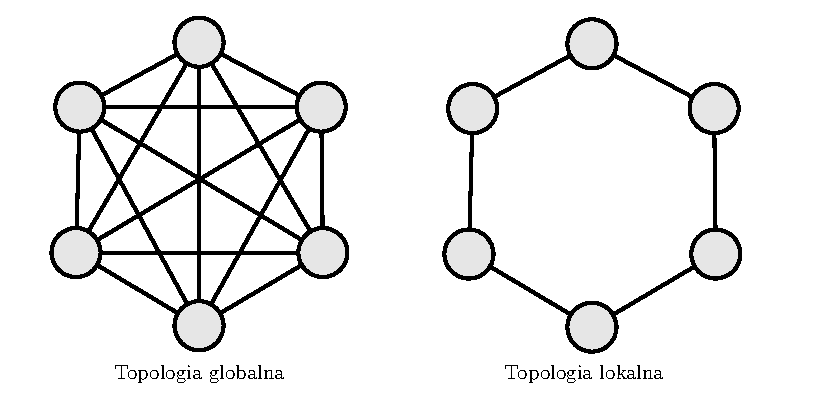
\includegraphics[width=\dimexpr.9\textwidth-1em]{grafiki/topologie.pdf}}
\captionof{figure}{Topologie widoczności rozwiązań i komunikacji między cząsteczkami.}
\label{fig:topologia}
\end{figure}

\subsection{Algorytm Monte Carlo} 

Metoda Monte Carlo opiera się na losowości wyboru położenia cząsteczek bez uwzględniania najlepszego globalnego położenia w całym roju. Cząsteczki zmieniają swoje położenie niezależnie od siebie. Położenie najlepszej cząsteczki $\vect{x}_{min}$ (o najmniejszej funkcji kosztu $f_{min} = f\left(\vect{x}_{min}\right)$) wyszukiwane jest tylko w celu znalezienia ostatecznego wyniku optymalizacji. Położenia cząstki w kolejnych generacjach w tym algorytmie można opisać zgodnie z następującym schematem
\begin{equation}
\vect{\overline{x}}_{i + 1, j} = \vect{x}_{i, j} + \sigma\vect{\xi},
\end{equation}
gdzie $\sigma$ to waga, a $\vect{\xi}$ to $n$-wymiarowa zmienna o rozkładzie jednostajnym. Zmienna $\vect{\overline{x}}_{i + 1, j}$ zostanie zaakceptowana jako nowa współrzędna cząstki $\vect{x}_{i + 1, j} = \vect{\overline{x}}_{i + 1, j}$, jeżeli funkcja celu $f\left(\vect{\overline{x}}_{i + 1, j}\right) < f\left(\vect{x}_{i, j}\right)$. W przeciwnym wypadku rozpatrywane są dwie możliwości.

Dodatkowo losowana jest zmienna $z$ o jednostajnym rozkładzie na przedziale $\left[0, \ 1 \right]$. Jeżeli spełniony będzie warunek
\begin{equation} \label{eq:mc_nie}
z < e^{-\frac{f\left(\vect{\overline{x}}_{i + 1, j}\right) - f\left(\vect{x}_{i, j}\right)}{T}},
\end{equation}
to nowe położenie, pomimo większej wartości funkcji celu, zostanie zaakceptowane ($T$ to parametr). Jeżeli nierówność (\ref{eq:mc_nie}) nie będzie spełniona, to cząstka w danej generacji nie zmieni swojego położenia $\vect{x}_{i + 1, j} = \vect{x}_{i, j}$. 

Literatura wskazuje, że na ogół lepiej jest wylosować wiele cząsteczek z całego zakresu i wykonać mniej iteracji niż oczekiwać spełnienia kryterium stopu przez jedną cząsteczkę pochodzącą z małej grupy cząstek. Przy dużym wymiarze wektora położenia może się okazać, że początkowo wylosowane cząsteczki nie znajdą się~w~basenach atrakcji wszystkich interesujących minimów. Wtedy przejście cząsteczek do innych basenów atrakcji może trwać wiele generacji i zależne będzie od wielkości parametru~$T$.

Należy zwrócić uwagę, że w podejściu Monte Carlo cząsteczki nie komunikują się - nie widzą swoich położeń i wartości funkcji celu nawzajem. Tym samym brak jest im inteligencji obserwowanej w PSO. Trajektoria każdej z cząsteczek w tym algorytmie zależy tylko od wylosowanych wartości zmiennych losowych.

Zastosowanie w zadaniach ograniczenia kostkowego i utrzymanie cząsteczek w obszarze dozwolonym zrealizowaliśmy identycznie jak w przypadku algorytmu PSO - odpowiedni wektor jest skalowany, aby nowe położenie spełniało ograniczenia. Podobnie, aby ujednolicić algorytmy, zastosowano takie same kryteria stopu.

\subsection{Zadania optymalizacji}
Zaimplementowane oprogramowanie będzie testowane poprzez rozwiązywanie następujących zadań optymalizacyjnych.
\subsubsection{Zadanie 1}
\begin{equation}
\min_{x} \left(f_{1}\left(\vect{x}\right) = \frac{1}{40} \sum_{i=1}^{n}\left(x_{i}\right)^{2} + 1 - \prod_{i =1}^{n} \cos\left(\frac{x_{i}}{i}\right)\right)
\end{equation}
\begin{equation}
-40 \leq x_{i} \leq 40 \quad i = 1, \ ..., \ n,
\end{equation}
gdzie minimum globalne $f_{\mathrm{min}} = 0$ w punkcie $\vect{x} = \vect{0}$.

\subsubsection{Zadanie 2}
\begin{equation}
\min_{x} \left(f_{2}\left(\vect{x}\right) = \sum_{i=1}^{n-1}\left(100\left(x_{i+1}-x_{i}^{2}\right)^{2} + \left(1-x_{i}\right)^{2} \right) \right)
\end{equation}
\begin{equation}
-40 \leq x_{i} \leq 40 \quad i = 1, \ ..., \ n,
\end{equation}
gdzie minimum globalne $f_{\mathrm{min}} = 0$ w punkcie $\vect{x} = \vect{1}$.

\section{Implementacja równoległa (OpenMP)}

W obydwu algorytmach zrównoleglenie polega na podziale liczby cząsteczek pomiędzy wątki. W~przypadku algorytmu Monte Carlo kolejne generacje cząsteczek mogą być obliczane niezależnie - cząsteczki są niezależne. W algorytmie optymalizacji rojem cząstek niezbędna jest synchronizacja - po~obliczeniu nowej generacji cząstek należy wybrać najlepszą z nich i umożliwić otrzymanie takiej informacji przez wszystkie pozostałe cząstki.

\subsection{Wersja równoległa PSO}

W metodzie optymalizacji rojem cząsteczek zrównoleglono dwa etapy algorytmu, tj. tworzenie roju cząsteczek (pętla \lstinline[style=mycpp]{for}) oraz obliczanie kolejnej generacji cząstek (zestaw instrukcji w pętli \lstinline[style=mycpp]{while}). Poniżej zamieszczone zostały fragmenty kodu odpowiedzialne za obliczanie kolejnej generacji cząstek przed (kod źródłowy \ref{code:pso_before}) oraz po (kod źródłowy \ref{code:pso_after}) zrównolegleniu. Możemy wyznaczyć kilka najważniejszych zmian wprowadzonych przez zastosowanie OpenMP:\nopagebreak
\begin{itemize}
\begin{samepage}
\item każdy wątek ma własny generator zmiennych losowych \lstinline[style=mycpp]{randEngine},
\end{samepage}
\item pętla aktualizująca położenia cząstek zrównoleglona jest dyrektywą \lstinline[style=mycpp]{#pragma omp for schedule(static)},
\item aktualizacja najlepszej cząstki wykonywana jest w sekcji krytycznej \lstinline[style=mycpp]{#pragma omp critical},
\item sprawdzenie warunku stopu wykonywane jest tylko przez jeden wątek \lstinline[style=mycpp]{#pragma omp single}.
\end{itemize}

\begin{lstlisting}[style=mycpp, label=code:pso_before, caption={Optymalizacja PSO - kod sekwencyjny.}]
std::default_random_engine randEngine;
rand_engine.seed(time(NULL));

int iterationNumber = 0;
while (configStop->computeStopCriterion(criterionStopValue,
	globalBestParticle))
{
    for (auto &singleParticle : particles)
    {
        singleParticle.computePosition(&rand_engine);
        updateBestParticle(&singleParticle);
    }
    iterationNumber++;
}
\end{lstlisting}

\begin{lstlisting}[style=mycpp, label=code:pso_after, caption={Optymalizacja PSO - kod równoległy.}]
bool foundSolution = false;
int iterationNumber = 0;
#pragma omp parallel
{
    std::default_random_engine randEngine;
    rand_engine.seed((omp_get_thread_num() + 1) * time(NULL));

    SwarmParticle *bestParticleInIteration = nullptr;

    while (!foundSolution)
    {
#pragma omp for schedule(static)
        for (int i = 0; i < amountOfParticles; i++)
        {
            particles[i].computePosition(&randEngine);

            if (bestParticleInIteration == nullptr)
                bestParticleInIteration = &particles[i];
            else if (particles[i].CostFunction() <
                        bestParticleInIteration->CostFunction())
                bestParticleInIteration = &particles[i];
        }

#pragma omp critical
        updateBestParticle(bestParticleInIteration);
        bestParticleInIteration = nullptr;

#pragma omp barrier

#pragma omp single
        {
            iterationNnumber++;

            if (!configStop->computeStopCriterion(criterionStopValue,
                    globalBestParticle))
                foundSolution = true;
        }
    }
}
\end{lstlisting}

\subsection{Wersja równoległa Monte Carlo}

Podobnie jak w metodzie PSO, w metodzie Monte Carlo zrównoleglono tworzenie cząsteczek oraz wyliczanie ich kolejnych generacji. Poniżej zamieszczono fragment kodu odpowiedzialny za obliczanie kolejnych generacji cząstek przed (kod źródłowy \ref{code:mc_before}) oraz po (kod źródłowy \ref{code:mc_after}) użyciu OpenMP. Zmiany kodu są analogiczne jak w przypadku algorytmu optymalizacji rojem cząsteczek.

\begin{lstlisting}[style=mycpp, label=code:mc_before, caption={Optymalizacja Monte Carlo - kod sekwencyjny.}]
std::default_random_engine randEngine;
rand_engine.seed(time(NULL));

int iterationNumber = 0;
while (configStop->computeStopCriterion(criterionStopValue,
    globalBestParticle))
{
    for (auto &particle : particles)
    {
        particle.computePosition(randEngine);
         updateBestParticle(&particle);
    }
    iterationNumber++;
}
\end{lstlisting}

\begin{lstlisting}[style=mycpp, label=code:mc_after, caption={Optymalizacja Monte Carlo - kod równoległy.}]
bool foundSolution = false;
int iterationNumber = 0;
int threadsCompleted = 0;
#pragma omp parallel
{
    std::default_random_engine randEngine;
    rand_engine.seed((omp_get_thread_num() + 1) * time(NULL));

    MonteCarloParticle *bestParticleInIteration = nullptr;

    int threads = omp_get_num_threads();

    while (!foundSolution)
    {
#pragma omp for schedule(static) nowait
        for (int i = 0; i < amountOfParticles; i++)
        {
            particles[i].computePosition(randEngine);

            if (bestParticleInIteration == nullptr)
                bestParticleInIteration = &particles[i];
            else if (particles[i].CostFunction() <
                        bestParticleInIteration->CostFunction())
                bestParticleInIteration = &particles[i];
        }

#pragma omp critical
        updateBestParticle(bestParticleInIteration);
        bestParticleInIteration = nullptr;

#pragma omp critical
        {
            threadsCompleted++;
            if (threadsCompleted >= threads)
            {
                threadsCompleted -= threads;
                iterationNumber++;

                if (!configStop->computeStopCriterion(criterionStopValue,
                        globalBestParticle))
                    foundSolution = true;
            }
        }
    }
}
\end{lstlisting}

\section{Sprzęt używany podczas testów} 

Testy przeprowadzono na komputerze, którego najważniejsze parametry zapisano w tabeli \ref{tab:parametry}.

\begin{table}[h]
\centering
\begin{tabular}{|l|l|}
\hline
Procesor          & Intel® Core™ i5-9600KF \\ \hline
Liczba rdzeni     & 6                              \\ \hline
Liczba wątków     & 6                              \\ \hline
Hyper-Threading   & Nie                                 \\ \hline
System operacyjny & Windows 10       \\ \hline
OpenMP			  & 4.5							        \\ \hline
\end{tabular}
\caption{Parametry używanego komputera.}
\label{tab:parametry}
\end{table}

\section{Kryterium stopu} \label{sec:stop}

Przyjęto dwa rodzaju warunków stopu nazywane dalej warunkiem akademickim oraz warunkiem normalnym. Warunek akademicki zakłada, że znana jest wartość minimum funkcji celu. W takim przypadku możemy uzależnić zakończenie optymalizacji od znalezienia położenia, które daje wynik dostatecznie bliski optymalnej wartości funkcji celu. W normalnych warunkach nie znamy wartości optimum, dlatego musimy zastosować inne kryteria zakończenia optymalizacji. Warunek akademicki jest czysto testowy i w większości dalej przeprowadzonych testów numerycznych będziemy się nim posługiwać.

W przypadku akademickiego warunku stopu wyliczana jest różnica pomiędzy wartością funkcji kosztu, a znanym a prori minimum funkcji. Następnie ta wartość porównywana jest z zadaną, satysfakcjonującą nas wartością przybliżenia optimum. Jeśli wyliczona różnica osiąga wartość równą bądź mniejszą niż podana, to optymalizacja kończy się i jako wynik podaje najlepsze położenie cząsteczki.

Normalny warunek stopu obliczany jest na podstawie zmian wartości funkcji celu najlepszych cząsteczek w $k$ ostatnich generacjach. Jeżeli zmiany są poniżej pewnego ustalonego poziomu $\tau$, to~algorytm optymalizacyjny kończy swoje działanie. W niekorzystnych przypadkach warunek może kończyć optymalizację zdecydowanie za szybko w związku z czym otrzymane wyniki należy traktować z~należytą niepewnością. Inne algorytmy dot. warunku normalnego wraz z porównaniem ich działania można znaleźć w \cite{karinZielinski}.

\subsection*{Test numeryczny normalnego kryterium stopu}

Dobór parametrów $k$ i $\tau$, które doprowadzą rozwiązanie zadania optymalizacji do zadowalającego przybliżenia optimum, jest bardzo trudny. W realiach optymalizacyjnych kształt i własności funkcji celu mogą być nieznane lub trudne do określenia. W tak niepewnym środowisku musimy znaleźć kompromis między długą i prawdopodobnie dokładną optymalizacją zmiennej decyzyjnej, a krótkim działaniem programu dającym jedynie zgrubne przybliżenie punktu optymalnego.

Trudności w zastosowaniu zaproponowanego wyżej normalnego kryterium stopu łatwo zaobserwować podczas stosowania algorytmu poszukiwań losowych. Jego praca, szczególnie w przypadku dużych wymiarów zadania, charakteryzuje się częstym tworzeniem wielu generacji cząstek, których położenia nie są lepsze od aktualnie znanego najlepszego punktu w przestrzeni. Tym samym, szybko dochodzi do~sytuacji, w której warunek normalny kończy działanie optymalizatora. Na rys. \ref{fig:warunek:mc} pokazano przykładowy przebieg optymalizacji - wartość funkcji celu w funkcji liczby generacji. Pokazana optymalizacja zadania $2$. zakończyła się kryterium stopu akademickiego (wartość funkcji celu poniżej $0.001$), lecz na wykresie oznaczono kółkami punkty zakończenia pracy optymalizatora w przypadku zastosowania warunku normalnego o oznaczonych parametrach.

\begin{figure}[h]
\centerline{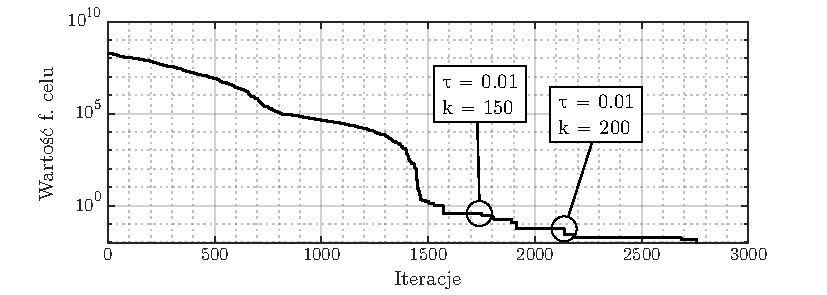
\includegraphics[width=\dimexpr.9\textwidth-1em]{grafiki/warunek_stopu.pdf}}
\captionof{figure}{Zakończenie optymalizacji normalnym kryterium stopu.}
\label{fig:warunek:mc}
\end{figure}

\section{Rozwiązanie zadań dla różnych wymiarów $n$}

W celu przetestowania i porównania algorytmów oraz ich implementacji rozwiązano zadania $1$. i $2$. w różnych wariantach. Zadania zostały rozwiązane zarówno przez wersje sekwencyjne programów, jak i wersje równoległe - utworzone z wykorzystaniem OpenMP. Wersje równoległe zostały uruchomione z~dostępnymi $6$ wątkami. Sprawdzono działanie programów w optymalizacji problemów o różnej złożoności, tj. każde z zadań zostało rozwiązane dla następujących wymiarów ($n$): $2, \ 10, \ 20, \ 50, \ 100$. Aby~ograniczyć działanie programu do czasów wykonywania poniżej $10$ minut, konieczne było w przypadkach o większym wymiarze problemu zwiększenie liczby cząsteczek.

W tabeli \ref{tab:rozw_zad1}. oraz tabeli \ref{tab:rozw_zad2}. przedstawiono wyniki serii testów odpowiednio dla zadania $1$. i $2$. Każdy test został wykonany co najmniej $10$ razy, aby móc uśrednić stochastyczny charakter algorytmów. W tabeli opracowano wyniki w postaci średniego, maksymalnego i minimalnego czasu wykonywania programu. Dołączono także wartość wariancji zebranych danych. Przedstawiony czas mierzony był dla części obliczeniowej programu, tj. dla samych obliczeń bez inicjalizacji potrzebnych zmiennych. Pomiary ograniczone były do czasu wykonywania pętli głównej symulacji.

Podczas uruchamiania algorytmu PSO użyto ustawień $\omega = \chi$, $c_1 = \chi c_1^*$, $c_2 = \chi c_2^*$, gdzie $\chi = 0.72984$, $c_1^* = c_2^* = 2.05$. W przypadku algorytmu Monte Carlo wybrano nastawy $\sigma = 0.1$, $T = 0.01$. W każdym przypadku położenia początkowe cząsteczek losowane z rozkładu jednostajnego na całym dozwolonym obszarze. Jako kryterium stopu przyjęto kryterium typu akademickiego z warunkiem zakończenia obliczeń $f\left(\vect{x}^{*}\right) < 0.01$.

Dla zadania $1$. wartość wariancji rośnie wraz ze wzrostem liczby cząsteczek. Do wymiaru $n = 20$ zwykle dla metody PSO wariancja jest mniejsza niż dla metody Monte Carlo. Natomiast dla wymiarów $n = 50$ i $n = 100$ sytuacja jest odwrotna. Dla cząsteczek o mniejszych wymiarach metoda PSO szybciej znajduje najlepszą cząsteczkę, a dla tych o większy wymiarach -- metoda Monte Carlo. Jest to~właściwość niezależna od zrównoleglenia. Wskazuje to na to, że \quotedblbase komunikacja\textquotedblright \ między cząsteczkami jest czasochłonna niezależnie czy obliczenia prowadzone są jednowątkowo czy wielowątkowo.

Dla zadania $2$., tak jak dla zadania $1$., wariancje rosną wraz z wymiarem przestrzeni. Niestety, dla~wymiarów $n=20$, $n=50$ i $n=100$ dla metody Monte Carlo i dla wymiaru $n=100$ dla metody PSO nie udało się dobrać parametrów tak, aby zadanie to liczyło się w dostatecznie krótkim czasie.

\renewcommand{\arraystretch}{2}
\begin{table}[t]
\scriptsize
\begin{adjustwidth}{-1.76cm}{}
\centering
\begin{tabular}{|c|c|c|l|l|l|l|l|l|l|l|l|l|}
\hline
\multicolumn{3}{|c|}{Wymiar}                                      & \multicolumn{2}{c|}{2}                             & \multicolumn{2}{c|}{10}                            & \multicolumn{2}{c|}{20}                            & \multicolumn{2}{c|}{50}                            & \multicolumn{2}{c|}{100}                           \\ \hline
\multicolumn{3}{|c|}{Algorytm}                                    & \multicolumn{1}{c|}{PSO} & \multicolumn{1}{c|}{MC} & \multicolumn{1}{c|}{PSO} & \multicolumn{1}{c|}{MC} & \multicolumn{1}{c|}{PSO} & \multicolumn{1}{c|}{MC} & \multicolumn{1}{c|}{PSO} & \multicolumn{1}{c|}{MC} & \multicolumn{1}{c|}{PSO} & \multicolumn{1}{c|}{MC} \\ \hline
\multicolumn{3}{|c|}{Liczba cząsteczek}                           & $10^{2}$                 & $10^{2}$                & $10^{2}$                 & $10^{2}$                & $10^{3}$                 & $10^{3}$                & $10^{3}$                 & $10^{3}$                & $10^{3}$                 & $10^{3}$                \\ \hline
\multirow{8}{*}{Czas} & \multirow{4}{*}{Sekwencyjnie} & Średnia   & $2.3 \ 10^{-4}$          & $1.1 \ 10^{-3}$         & $2.4 \ 10^{-3}$          & $2.9 \ 10^{-1}$         & $2.9 \ 10^{-2}$          & $1.1 \ 10^{0}$          & $1.5 \ 10^{2}$           & $3.1 \ 10^{1}$          & $4.9 \ 10^{2}$           & $8.6 \ 10^{1}$          \\ \cline{3-13} 
                      &                               & Minimum   & $1.9 \ 10^{-4}$          & $3.1 \ 10^{-4}$         & $2.8 \ 10^{-3}$          & $2.2 \ 10^{-1}$         & $2.6 \ 10^{-2}$          & $9.5 \ 10^{-1}$          & $8.3 \ 10^{1}$           & $2.8 \ 10^{1}$          & $2.3 \ 10^{2}$           & $8.0 \ 10^{1}$          \\ \cline{3-13} 
                      &                               & Maksimum  & $5.0 \ 10^{-4}$          & $1.6 \ 10^{-3}$         & $3.1 \ 10^{-3}$          & $3.5 \ 10^{-1}$         & $3.1 \ 10^{-2}$          & $1.2 \ 10^{0}$          & $2.4 \ 10^{2}$           & $3.3 \ 10^{1}$          & $7.4 \ 10^{2}$           & $9.3 \ 10^{1}$          \\ \cline{3-13} 
                      &                               & Wariancja & $6.6 \ 10^{-9}$          & $2.0 \ 10^{-7}$         & $4.6 \ 10^{-8}$          & $1.4 \ 10^{-3}$         & $1.1 \ 10^{-6}$          & $2.4 \ 10^{-3}$         & $2.2 \ 10^{3}$           & $1.8 \ 10^{0}$          & $2.2 \ 10^{2}$           & $1.6 \ 10^{1}$          \\ \cline{2-13} 
                      & \multirow{4}{*}{Równolegle}   & Średnia   & $7.3 \ 10^{-5}$          & $2.1 \ 10^{-4}$         & $6.6 \ 10^{-4}$          & $5.5 \ 10^{-2}$         & $9.7 \ 10^{-3}$          & $1.9 \ 10^{-1}$         & $3.4 \ 10^{1}$           & $5.1 \ 10^{0}$          & $8.2 \ 10^{1}$           & $1.4 \ 10^{1}$          \\ \cline{3-13} 
                      &                               & Minimum   & $5.3 \ 10^{-5}$          & $2.0 \ 10^{-4}$         & $4.8 \ 10^{-4}$          & $4.7 \ 10^{-2}$         & $4.7 \ 10^{-3}$          & $1.7 \ 10^{-1}$         & $7.6 \ 10^{0}$           & $4.9 \ 10^{0}$          & $5.9 \ 10^{1}$           & $1.3 \ 10^{1}$          \\ \cline{3-13} 
                      &                               & Maksimum  & $1.6 \ 10^{-4}$          & $3.4 \ 10^{-4}$         & $4.6 \ 10^{-3}$          & $7.9 \ 10^{-2}$         & $5.6 \ 10^{-2}$          & $2.4 \ 10^{-1}$          & $5.7 \ 10^{1}$           & $5.4 \ 10^{0}$          & $1.2 \ 10^{2}$           & $1.5 \ 10^{1}$          \\ \cline{3-13} 
                      &                               & Wariancja & $6.3 \ 10^{-10}$         & $2.4 \ 10^{-10}$        & $5.4 \ 10^{-7}$          & $6.4 \ 10^{-5}$         & $1.2 \ 10^{-4}$          & $1.9 \ 10^{-4}$         & $2.4 \ 10^{2}$           & $1.9 \ 10^{-2}$         & $5.4 \ 10^{2}$           & $1.4 \ 10^{-1}$         \\ \hline
\end{tabular}
\end{adjustwidth}
\caption{Rozwiązania zadania $1$. dla różnych wymiarów $n$ i ustawień.}
\label{tab:rozw_zad1}
\end{table}

\begin{table}[t]
\scriptsize
\begin{adjustwidth}{.7cm}{}
\centering
\begin{tabular}{|c|c|c|l|l|l|l|l|c|l|c|c|c|}
\hline
\multicolumn{3}{|c|}{Wymiar}                                      & \multicolumn{2}{c|}{2}                             & \multicolumn{2}{c|}{10}                            & \multicolumn{2}{c|}{20}                                  & \multicolumn{2}{c|}{50}                                  & \multicolumn{2}{c|}{100}                                      \\ \hline
\multicolumn{3}{|c|}{Algorytm}                                    & \multicolumn{1}{c|}{PSO} & \multicolumn{1}{c|}{MC} & \multicolumn{1}{c|}{PSO} & \multicolumn{1}{c|}{MC} & \multicolumn{1}{c|}{PSO} & MC                            & \multicolumn{1}{c|}{PSO} & MC                            & PSO                           & MC                            \\ \hline
\multicolumn{3}{|c|}{Liczba cząsteczek}                           & $10^{2}$                 & $10^{2}$                & $10^{2}$                 & $10^{2}$                & $10^{2}$                 & \multicolumn{1}{l|}{$10^{2}$} & $10^{4}$                 & \multicolumn{1}{l|}{$10^{4}$} & \multicolumn{1}{l|}{$10^{3}$} & \multicolumn{1}{l|}{$10^{3}$} \\ \hline
\multirow{8}{*}{Czas} & \multirow{4}{*}{Sekwencyjnie} & Średnia   & $1.3 \ 10^{-3}$          & $4.3 \ 10^{-3}$         & $6.3 \ 10^{-2}$          & $1.9 \ 10^{1}$          & $1.2 \ 10^{0}$           & -                             & $3.8 \ 10^{2}$           & -                             & -                             & -                             \\ \cline{3-13} 
                      &                               & Minimum   & $1.3 \ 10^{-3}$          & $3.3 \ 10^{-3}$         & $5.4 \ 10^{-2}$          & $1.3 \ 10^{1}$          & $8.9 \ 10^{-1}$          & -                             & $3.1 \ 10^{2}$           & -                             & -                             & -                             \\ \cline{3-13} 
                      &                               & Maksimum  & $1.5 \ 10^{-3}$          & $5.5 \ 10^{-3}$         & $7.5 \ 10^{-2}$          & $2.8 \ 10^{1}$          & $1.9 \ 10^{0}$           & -                             & $4.4 \ 10^{2}$           & -                             & -                             & -                             \\ \cline{3-13} 
                      &                               & Wariancja & $4.1 \ 10^{-9}$          & $5.9 \ 10^{-7}$         & $7.5 \ 10^{-5}$          & $2.1 \ 10^{1}$          & $5.6 \ 10^{-2}$          & -                             & $2.6 \ 10^{3}$           & -                             & -                             & -                             \\ \cline{2-13} 
                      & \multirow{4}{*}{Równolegle}   & Średnia   & $4.7 \ 10^{-4}$          & $8.8 \ 10^{-4}$         & $1.7 \ 10^{-2}$          & $3.1 \ 10^{0}$          & $2.8 \ 10^{-1}$          & -                             & $5.4 \ 10^{1}$           & -                             & -                             & -                             \\ \cline{3-13} 
                      &                               & Minimum   & $3.1 \ 10^{-4}$          & $8.5 \ 10^{-4}$         & $1.2 \ 10^{-2}$          & $1.9 \ 10^{0}$          & $1.7 \ 10^{-1}$          & -                             & $3.7 \ 10^{1}$           & -                             & -                             & -                             \\ \cline{3-13} 
                      &                               & Maksimum  & $4.4 \ 10^{-3}$          & $9.8 \ 10^{-4}$         & $1.4 \ 10^{-1}$          & $5.2 \ 10^{0}$          & $4.7 \ 10^{-1}$          & -                             & $6.4 \ 10^{1}$           & -                             & -                             & -                             \\ \cline{3-13} 
                      &                               & Wariancja & $5.5 \ 10^{-7}$          & $6.7 \ 10^{-10}$        & $5.8 \ 10^{-4}$          & $1.2 \ 10^{0}$          & $4.5 \ 10^{-1}$          & -                             & $8.4 \ 10^{1}$           & -                             & -                             & -                             \\ \hline
\end{tabular}
\end{adjustwidth}
\caption{Rozwiązania zadania $2$. dla różnych wymiarów $n$ i ustawień.}
\label{tab:rozw_zad2}
\end{table}
\renewcommand{\arraystretch}{1}

\newpage

\begin{figure}[H]
\centering
\begin{minipage}[b]{\dimexpr.5\textwidth-1em}
  \centering
  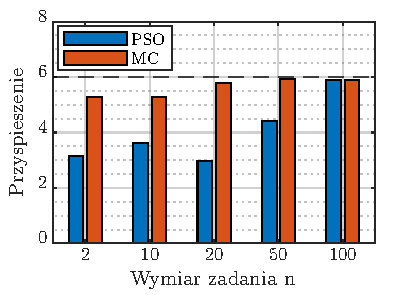
\includegraphics[width=1\linewidth]{grafiki/tabela_zad1_przyspieszenie.pdf}
  \captionof{figure}{Średnie przyspieszenie implementacji równoległej podczas prób optymalizacji zad. $1$.}
  \label{fig:przysp:zad1}
\end{minipage} \hfill
\begin{minipage}[b]{\dimexpr.5\textwidth-1em}
  \centering
  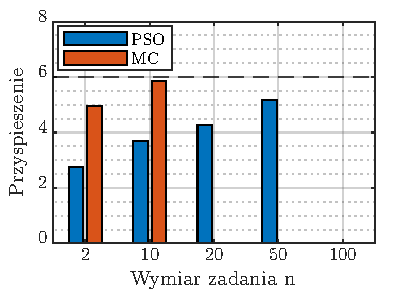
\includegraphics[width=1\linewidth]{grafiki/tabela_zad2_przyspieszenie.pdf}
  \captionof{figure}{Średnie przyspieszenie implementacji równoległej podczas prób optymalizacji zad. $2$.}
  \label{fig:przysp:zad2}
\end{minipage}
\end{figure}

Na wykresach z rys. \ref{fig:przysp:zad1} i \ref{fig:przysp:zad2} zebrano uzyskane przyspieszenia obliczeń wersji równoległej względem sekwencyjnej w zależności od wymiaru rozwiązywanego zadania. Widoczne jest, że tendencja powiązania przyspieszenia z wymiarem jest zachowana w obu testowanych zadaniach. Można przypuszczać, że~duże zmiany przyspieszenia dla~małych wymiarów w~przypadku algorytmu PSO wynikają z~większego udziału w~całkowitym czasie obliczeń oczekiwania na~odblokowanie sekcji krytycznych, w~których odbywa się~synchronizacja wiedzy na~temat najlepszej cząsteczki.

\section{Ocena skalowalności}

Zbadano skalowalność implementacji oraz przyspieszenie wynikające z użycia obliczeń równoległych. Wykonano $4$ testy - dla każdej metody zbadano czasy wykonywania obliczeń przy optymalizacji zadania $1$. oraz zadania $2$. Opcje konfiguracyjne algorytmów i ustawienia ilości cząsteczek oraz wymiarów zadań były stałe podczas pojedynczego testu. Zmianom ulegała liczba dostępnych wątków programu.

W każdym teście położenia początkowe cząsteczek wylosowane zostały z obszaru ograniczonego nierównościami $-40 \leq x_i \leq -30 \quad i = 1, \ ...\, \ n$, aby uniknąć sytuacji, w której pewne cząstki w swojej początkowej konfiguracji spełniają kryterium stopu lub znajdują się bardzo blisko poszukiwanego rozwiązania. W testach użyto kryterium stopu akademickiego z warunkiem zakończenia $f\left(\vect{x}^{*}\right) < 0.01$.

Wyniki testu paralelizacji algorytmu optymalizacji rojem cząstek dla optymalizacji zadania $1$. oraz $2$. pokazano odpowiednio na rys. \ref{fig:skalowalnosc:PSO1} i rys. \ref{fig:skalowalnosc:PSO2}. W testach użyto ustawień $\omega = \chi$, $c_1 = \chi c_1^*$, $c_2 = \chi c_2^*$, gdzie $\chi = 0.72984$, $c_1^* = c_2^* = 2.05$.

Wyniki testu paralelizacji algorytmu Monte Carlo dla zadania $1$. oraz $2$. pokazano odpowiednio na rys. \ref{fig:skalowalnosc:MC1} i rys. \ref{fig:skalowalnosc:MC2}. Rozwiązując zadanie $1$ użyto ustawień $\sigma = 1$, $T = 0.01$, a podczas rozwiązywania zadania $2$ parametry algorytmu ustawiono na $\sigma = 0.1$, $T = 0.01$.

\begin{figure}[h]
\centering
\begin{minipage}[b]{\dimexpr.5\textwidth-1em}
  \centering
  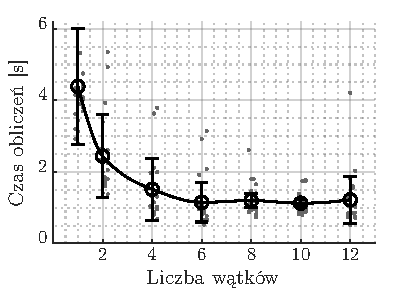
\includegraphics[width=1\linewidth]{grafiki/skalowalnosc_PSO_z1.pdf}
  \captionof{figure}{Test skalowalności algorytmu PSO na przykładzie optymalizacji zadania $1$. o $n = 20$ wymiarach. Użyto $10^{5}$ cząstek.}
  \label{fig:skalowalnosc:PSO1}
\end{minipage} \hfill
\begin{minipage}[b]{\dimexpr.5\textwidth-1em}
  \centering
  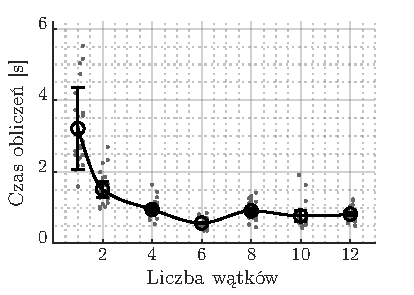
\includegraphics[width=1\linewidth]{grafiki/skalowalnosc_PSO_z2.pdf}
  \captionof{figure}{Test skalowalności algorytmu PSO na przykładzie optymalizacji zadania $2$. o $n = 10$ wymiarach. Użyto $10^{5}$ cząstek.}
  \label{fig:skalowalnosc:PSO2}
\end{minipage}
\end{figure}

\begin{figure}[h]
\centering
\begin{minipage}[b]{\dimexpr.5\textwidth-1em}
  \centering
  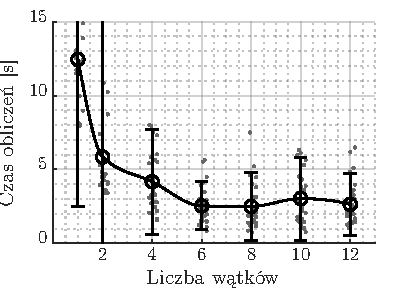
\includegraphics[width=1\linewidth]{grafiki/skalowalnosc_MC_z1.pdf}
  \captionof{figure}{Test skalowalności algorytmu MC na przykładzie optymalizacji zadania $1$. o $n = 10$ wymiarach. Użyto $10^{5}$ cząstek.}
  \label{fig:skalowalnosc:MC1}
\end{minipage} \hfill
\begin{minipage}[b]{\dimexpr.5\textwidth-1em}
  \centering
  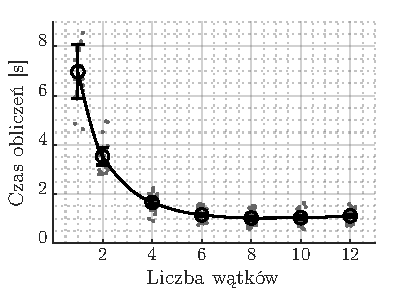
\includegraphics[width=1\linewidth]{grafiki/skalowalnosc_MC_z2.pdf}
  \captionof{figure}{Test skalowalności algorytmu MC na przykładzie optymalizacji zadania $2$. o $n = 4$ wymiarach. Użyto $10^{4}$ cząstek.}
  \label{fig:skalowalnosc:MC2}
\end{minipage}
\end{figure}

\section{Porównanie trajektorii dla $n = 2$}

%Funkcja kosztu - zad1 i zad2
\begin{figure}[H]
\centerline{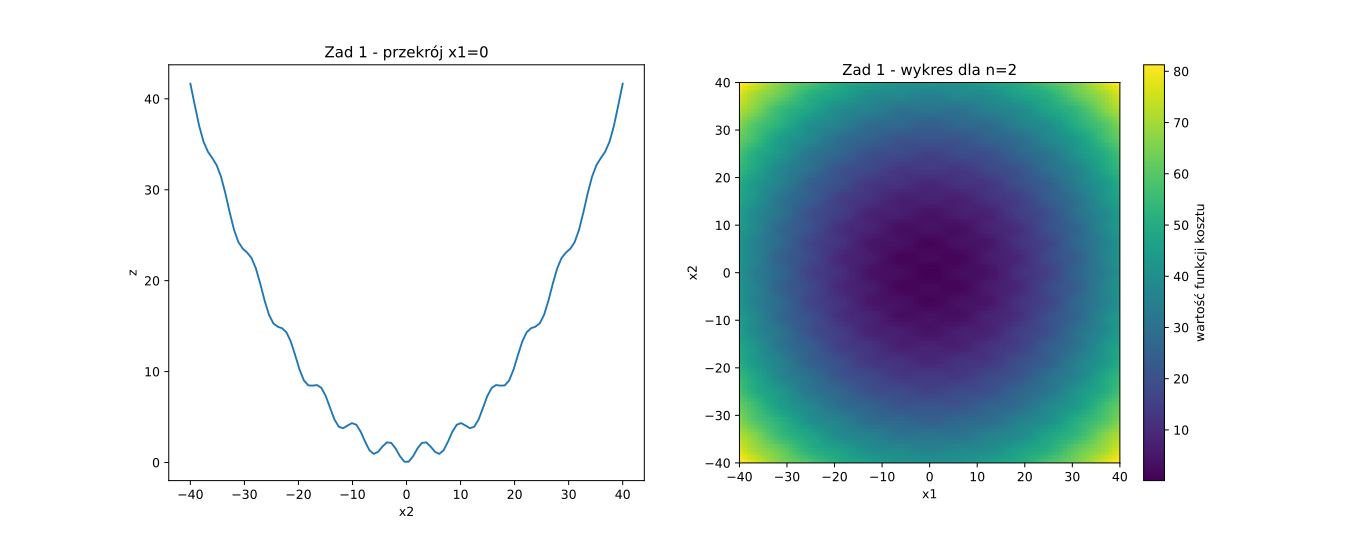
\includegraphics[width=\dimexpr.9\textwidth-1em]{grafiki//Wykresy2d/Zad1_2d_heatmap.png}}
\captionof{figure}{Wartość funkcji kosztu dla zadania $1$.}
\label{fig:zad1:koszt2d}
\end{figure}

\begin{figure}[H]
\centerline{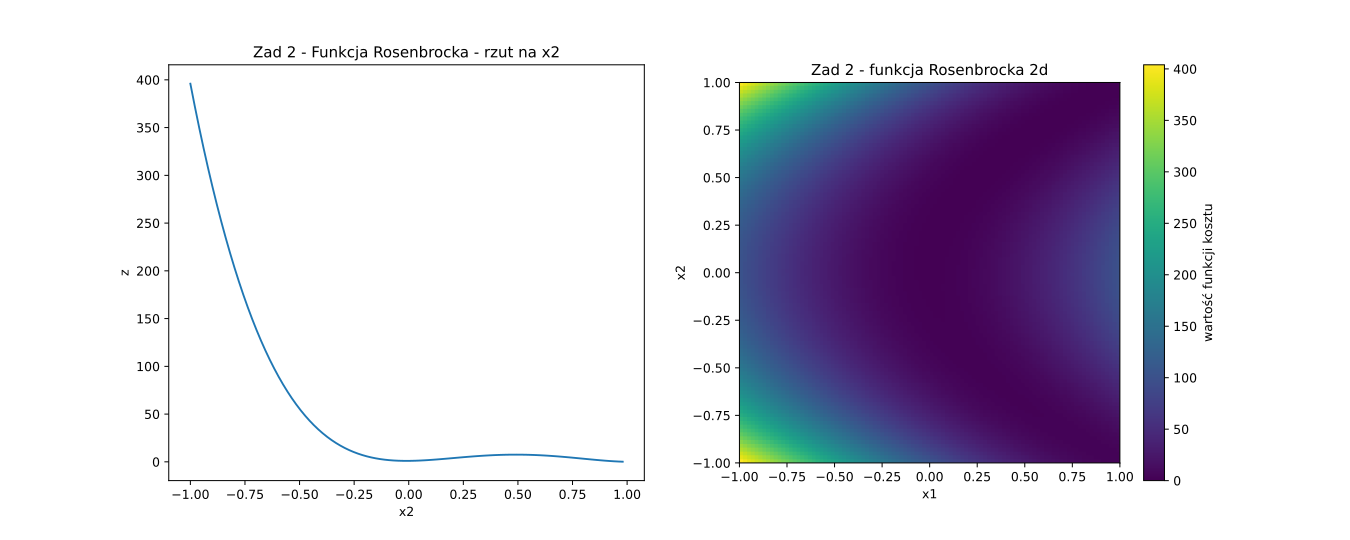
\includegraphics[width=\dimexpr.9\textwidth-1em]{grafiki//Wykresy2d/Rosenbrock_2d_heatmap_close_min.png}}
\captionof{figure}{Wartość funkcji kosztu dla zadania $2$. - obszar blisko minimum globalnego.}
\label{fig:zad1:koszt2d}
\end{figure}

%Pozycje startowe
\begin{figure}[H]
\centering
\begin{minipage}[b]{\dimexpr.5\textwidth-1em}
  \centering
  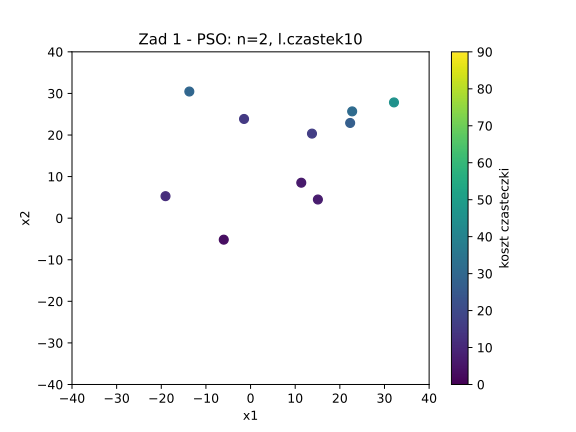
\includegraphics[width=1\linewidth]{grafiki/Wykresy2d/PSO_zad1_startPositions.png}
  \captionof{figure}{Pozycje startowe cząsteczek dla algorytmu PSO dla zadania $1$.}
  \label{fig:pozycjeStartowe:PSO1}
\end{minipage} \hfill
\begin{minipage}[b]{\dimexpr.5\textwidth-1em}
  \centering
  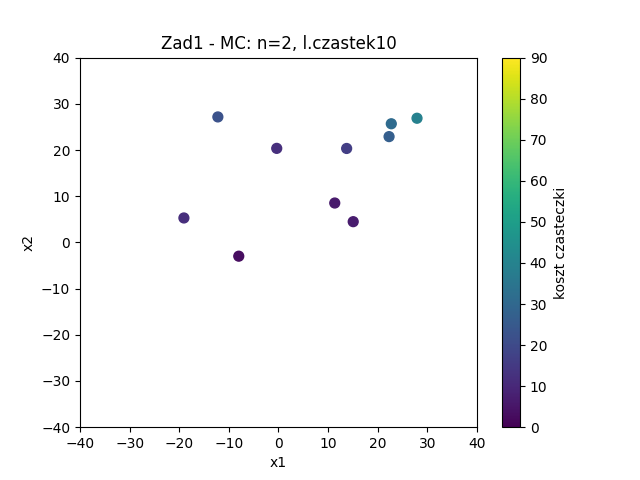
\includegraphics[width=1\linewidth]{grafiki/Wykresy2d/MC_Zad1_startPositions.png}
  \captionof{figure}{Pozycje startowe cząsteczek dla algorytmu MC dla zadania $1$.}
  \label{fig:pozycjeStartowe:MC1}
\end{minipage}
\end{figure}

\begin{figure}[H]
\centering
\begin{minipage}[b]{\dimexpr.5\textwidth-1em}
  \centering
  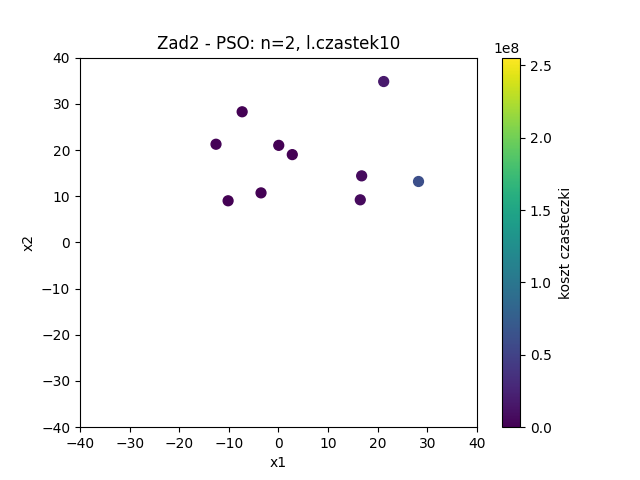
\includegraphics[width=1\linewidth]{grafiki/Wykresy2d/PSO_Zad2_startPositions.png}
  \captionof{figure}{Pozycje startowe cząsteczek dla algorytmu PSO dla zadania $2$.}
  \label{fig:pozycjeStartowe:PSO2}
\end{minipage} \hfill
\begin{minipage}[b]{\dimexpr.5\textwidth-1em}
  \centering
  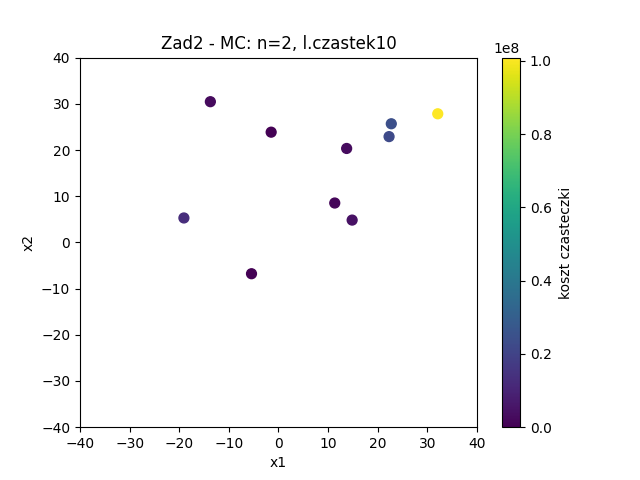
\includegraphics[width=1\linewidth]{grafiki/Wykresy2d/MC_Zad2_startPositions.png}
  \captionof{figure}{Pozycje startowe cząsteczek dla algorytmu MC dla zadania $2$.}
  \label{fig:pozycjeStartowe:MC2}
\end{minipage}
\end{figure}

% Położenia dla wszystkich iteracji

\begin{figure}[H]
\centering
\begin{minipage}[b]{\dimexpr.5\textwidth-1em}
  \centering
  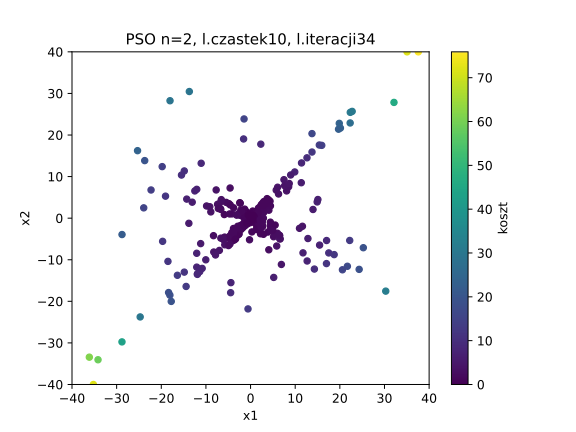
\includegraphics[width=1\linewidth]{grafiki/Wykresy2d/PSO_zad1_scatter_allIters.png}
  \captionof{figure}{Położenia wszystkich cząsteczek dla algorytmu PSO dla zadania $1$.}
  \label{fig:położeniaWszystkich:PSO1}
\end{minipage} \hfill
\begin{minipage}[b]{\dimexpr.5\textwidth-1em}
  \centering
  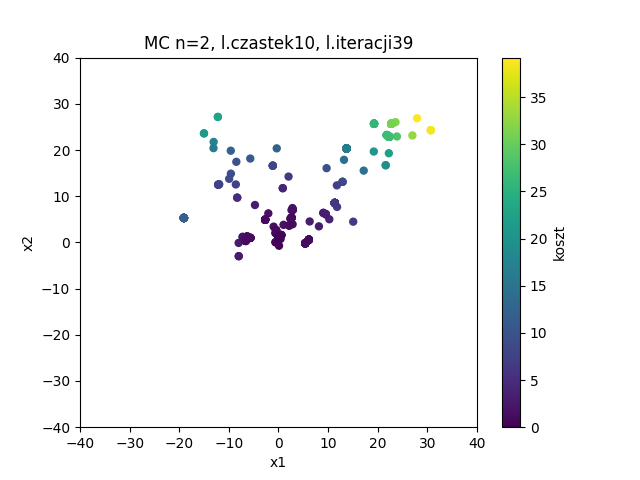
\includegraphics[width=1\linewidth]{grafiki/Wykresy2d/MC_Zad1_scatter_allIters.png}
  \captionof{figure}{Położenia wszystkich cząsteczek dla algorytmu MC dla zadania $1$.}
  \label{fig:położeniaWszystkich:MC1}
\end{minipage}
\end{figure}

\begin{figure}[H]
\centering
\begin{minipage}[b]{\dimexpr.5\textwidth-1em}
  \centering
  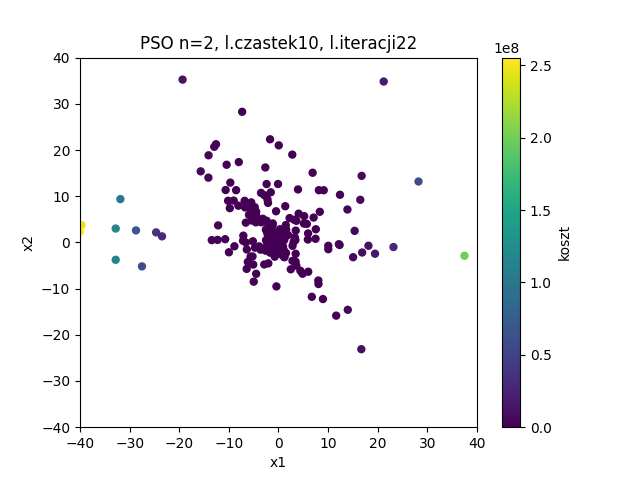
\includegraphics[width=1\linewidth]{grafiki/Wykresy2d/PSO_Zad2_scatter_allIters.png}
  \captionof{figure}{Położenia wszystkich cząsteczek dla algorytmu PSO dla zadania $2$.}
  \label{fig:położeniaWszystkich:PSO2}
\end{minipage} \hfill
\begin{minipage}[b]{\dimexpr.5\textwidth-1em}
  \centering
  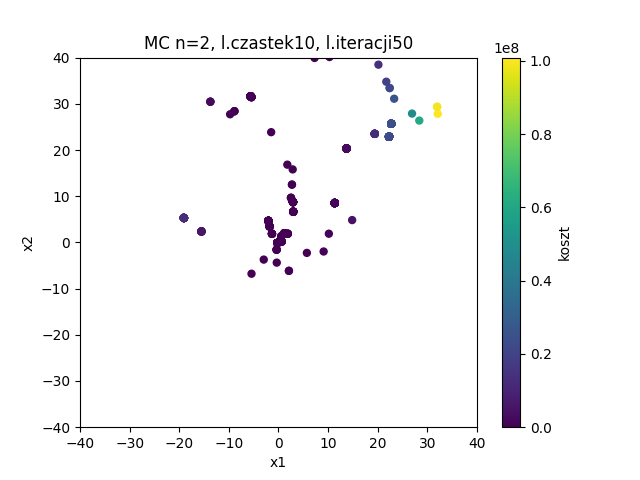
\includegraphics[width=1\linewidth]{grafiki/Wykresy2d/MC_Zad2_scatter_allIters.png}
  \captionof{figure}{Położenia wszystkich cząsteczek dla algorytmu MC dla zadania $2$.}
  \label{fig:położeniaWszystkich:MC2}
\end{minipage}
\end{figure}

% Trajektoria wybranej cząstki

\begin{figure}[H]
\centering
\begin{minipage}[b]{\dimexpr.5\textwidth-1em}
  \centering
  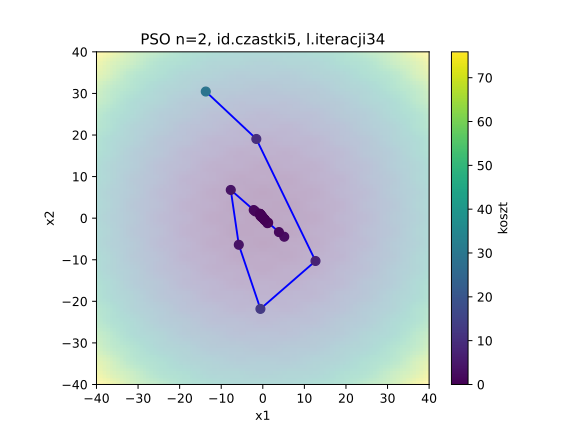
\includegraphics[width=1\linewidth]{grafiki/Wykresy2d/zad1_pso_plot_5.png}
  \captionof{figure}{Trajektoria wybranej cząstki dla algorytmu PSO dla zadania $1$.}
  \label{fig:trajektoriaWybrana:PSO1}
\end{minipage} \hfill
\begin{minipage}[b]{\dimexpr.5\textwidth-1em}
  \centering
  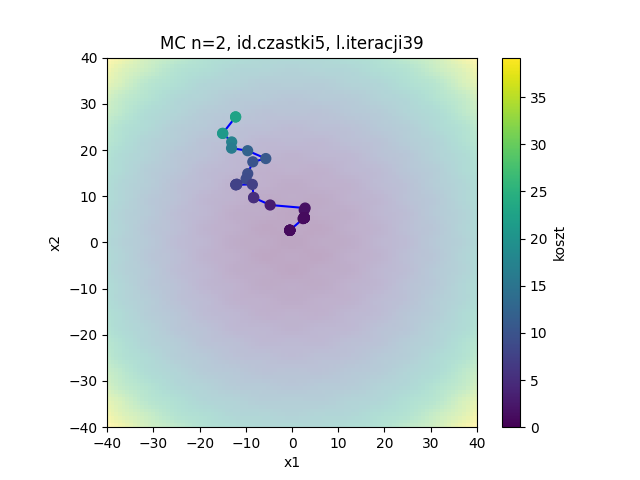
\includegraphics[width=1\linewidth]{grafiki/Wykresy2d/Zad1_MC_plot_5.png}
  \captionof{figure}{Trajektoria wybranej cząstki dla algorytmu MC dla zadania $1$.}
  \label{fig:trajektoriaWybrana:MC1}
\end{minipage}
\end{figure}

\begin{figure}[H]
\centering
\begin{minipage}[b]{\dimexpr.5\textwidth-1em}
  \centering
  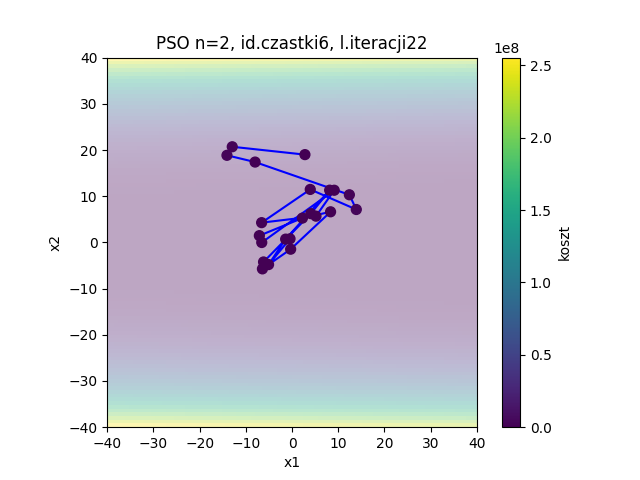
\includegraphics[width=1\linewidth]{grafiki/Wykresy2d/Zad2_PSO_plot_6.png}
  \captionof{figure}{Trajektoria wybranej cząstki dla algorytmu PSO dla zadania $2$.}
  \label{fig:trajektoriaWybrana:PSO2}
\end{minipage} \hfill
\begin{minipage}[b]{\dimexpr.5\textwidth-1em}
  \centering
  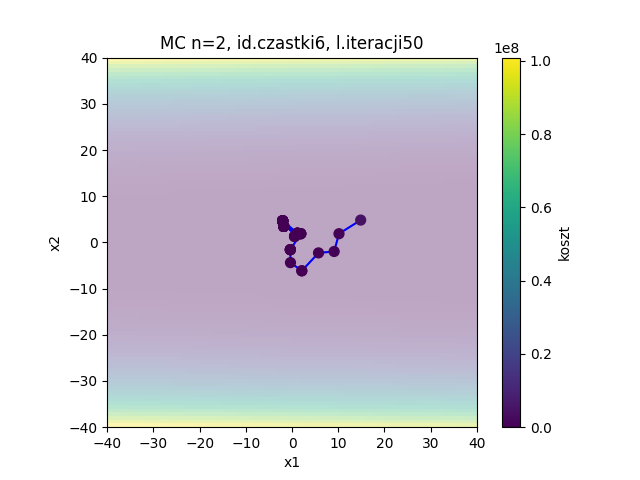
\includegraphics[width=1\linewidth]{grafiki/Wykresy2d/Zad2_MC_plot_6.png}
  \captionof{figure}{Trajektoria wybranej cząstki dla algorytmu MC dla zadania $2$.}
  \label{fig:trajektoriaWybrana:MC2}
\end{minipage}
\end{figure}

% Położenia najlepszego rozwiązania dla kazdej iteracji

\begin{figure}[H]
\centering
\begin{minipage}[b]{\dimexpr.5\textwidth-1em}
  \centering
  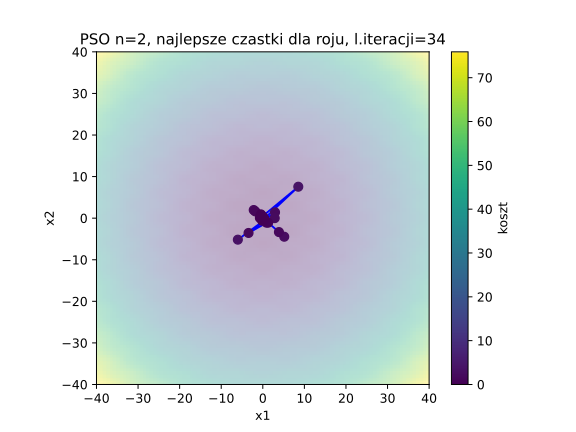
\includegraphics[width=1\linewidth]{grafiki/Wykresy2d/zad1_pso_plot_BEST.png}
  \captionof{figure}{Położenia najlepszego rozwiązania w~każdej z iteracji dla algorytmu PSO dla zadania $1$.}
  \label{fig:najepszeRozwiazanie:PSO1}
\end{minipage} \hfill
\begin{minipage}[b]{\dimexpr.5\textwidth-1em}
  \centering
  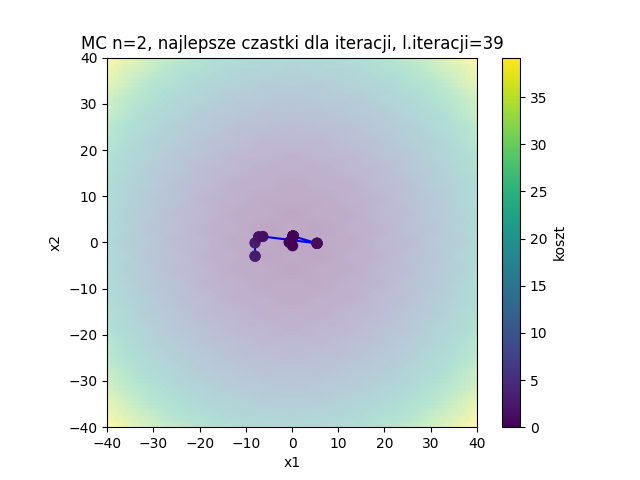
\includegraphics[width=1\linewidth]{grafiki/Wykresy2d/Zad1_MC_plot_BEST.png}
  \captionof{figure}{Położenia najlepszego rozwiązania w~każdej z iteracji dla algorytmu MC dla zadania $1$.}
  \label{fig:najepszeRozwiazanie:MC1}
\end{minipage}
\end{figure}

\begin{figure}[H]
\centering
\begin{minipage}[b]{\dimexpr.5\textwidth-1em}
  \centering
  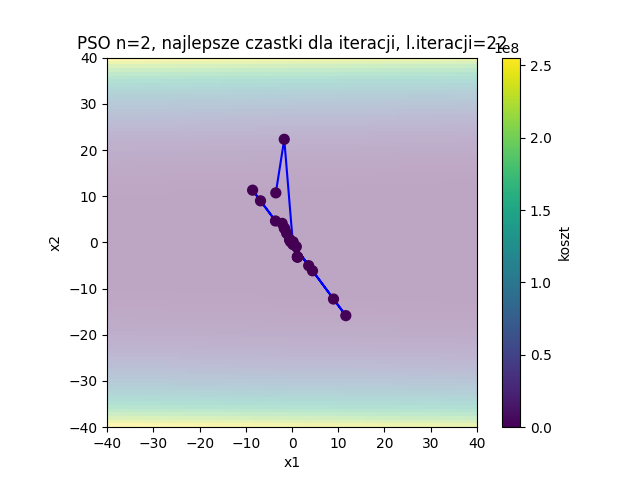
\includegraphics[width=1\linewidth]{grafiki/Wykresy2d/Zad2_PSO_plot_BEST.png}
  \captionof{figure}{Położenia najlepszego rozwiązania w każdej z iteracji dla algorytmu PSO dla zadania $2$.}
  \label{fig:najepszeRozwiazanie:PSO2}
\end{minipage} \hfill
\begin{minipage}[b]{\dimexpr.5\textwidth-1em}
  \centering
  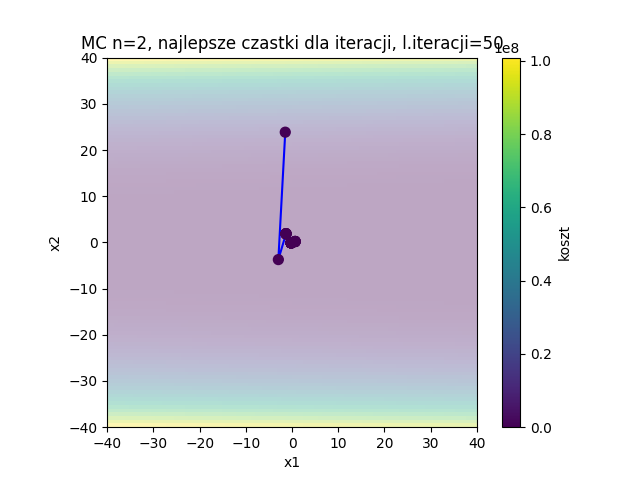
\includegraphics[width=1\linewidth]{grafiki/Wykresy2d/Zad2_MC_plot_BEST.png}
  \captionof{figure}{Położenia najlepszego rozwiązania w każdej z iteracji dla algorytmu MC dla zadania $2$.}
  \label{fig:najepszeRozwiazanie:MC2}
\end{minipage}
\end{figure}

Z wykresów trajektorii dla cząsteczki o wymiarze $n=2$ widać, ze cząsteczki obliczane z użyciem algorytmu PSO bardzo ładnie schodzą się w stronę globalnego minimum. Dla metody Monte Carlo takiej obserwacji nie można poczynić. Jednocześnie widać, że Przy obliczeniach dla metody PSO potrzebne jest mniej iteracji niż przy metodzie Monte Carlo aby otrzymać satysfakcjonujący wynik.

\section{Profil zbieżności algorytmów}

Postanowiono również porównać zbieżność omawianych metod na przykładowym zadaniu. W tym teście dodano także wariant metody PSO - metodę lokalną (oznaczaną na wykresach jako \textit{PSO Local}). Dane wykorzystane w tym badaniu pochodziły z prób optymalizacji zadania $2.$ (funkcja Rosenbrocka) o wymiarze $n = 4$ i ustalonej liczbie cząsteczek $10^{4}$. Ostateczny profil zbieżności dla każdej z metod powstał z normalizacji liczby iteracji do $100$ oraz uśrednienia tak znormalizowanych przebiegów zbieżności z $10$ prób.

W testach z metodą PSO (zarówno wariant globalny jak i lokalny) użyto następujących parametrów $\omega = \chi$, $c_1 = \chi c_1^*$, $c_2 = \chi c_2^*$, gdzie $\chi = 0.72984$, $c_1^* = c_2^* = 2.05$. Algorytm poszukiwań losowych działał natomiast z ustawieniami $\sigma = 0.1$, $T = 0.01$. Pozycje początkowe cząstek losowano z ograniczeniem $-40 \leq x_i \leq -30 \quad i = 1, \ ...\, \ n$. Obie metody włączane były w wersji równoległej z~$6$~wątkami.

Tak utworzony profil zbieżności przedstawiono na rys. \ref{fig:zbieznosc}. Widoczna jest znaczna różnica w początkowym zachowaniu algorytmu lokalnego PSO. Po około $30$ iteracjach profil zbieżności jest niemal identyczny dla każdego z podejść. Należy jednak pamiętać, że wykres ten nie odzwierciedla różnic w czasie obliczeń. Pod tym względem najlepszą metodą była metoda globalna PSO, a najsłabszą podejście Monte Carlo.

\begin{figure}[h]
\centerline{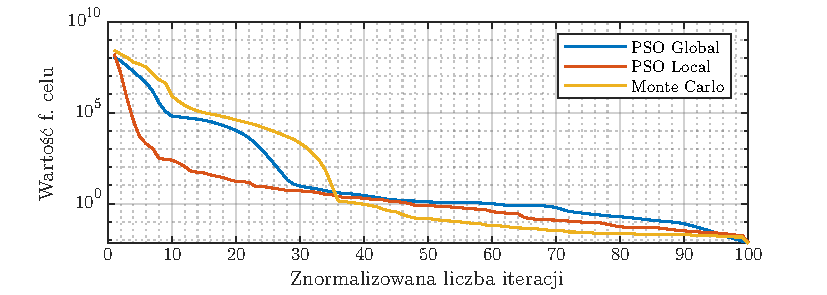
\includegraphics[width=\dimexpr.9\textwidth-1em]{grafiki/zbieznosc_porownanie.pdf}}
\captionof{figure}{Porównanie zbieżności algorytmów dla przykładowego zadania optymalizacji.}
\label{fig:zbieznosc}
\end{figure}

\vspace{-.8cm}
\section{Wnioski} 

Niestety nie ma możliwości wykonać obu zadań dla obu algorytmów dokładnie z tymi samymi ustawieniami tak, aby w łatwy sposób porównać ich działanie. Wraz z zwiększaniem wymiaru zadania zwiększano również liczbę cząstek, co, jak zauważono, pozytywnie wpływało na czas obliczeń. Oprócz liczby cząsteczek przeszukujących zadany obszar zmianom ulegały parametry algorytmów. Ich~dobieranie wykonywane było na zasadzie prób i błędów.

Tak jak można było przypuszczać zarówno dla zadania $1$, jak i $2$. dla obu rodzajów algorytmów zrównoleglenie fragmentów kodu przyspieszyło działanie programu (rys. \ref{fig:skalowalnosc:PSO1}, rys. \ref{fig:skalowalnosc:PSO2}, rys. \ref{fig:skalowalnosc:MC1} i rys. \ref{fig:skalowalnosc:MC2}). Okazało się również, że przyspieszenie to następuje dla liczby wątków nie większej niż liczba rdzeni, czyli $6$. Gdy obliczenia wykonywane są na większej liczbie wątków niż liczba rdzeni, czas szukania najlepszej cząstki jest porównywalny z czasem szukania tej cząstki na $6$ rdzeniach. Nie widać natomiast, aby po przekroczeniu granicy $6$ wątków następowały jakieś większe problemy w komunikacji między wątkami.

Największe przyspieszenie, niezależnie od rodzaju zadania czy rodzaju algorytmu, występuje pomiędzy użyciem $1$ a $2$ wątków. Przy włączeniu kolejnych wątków (aż do $6$ granicznych) różnica w~czasie obliczeń jest coraz mniejsza.

Dla algorytmu Monte Carlo przy dłuższym czasie wykonywania obliczeń, korzyść ze zrównleglenia jest większa niż dla PSO. Jest to zapewne wynikiem tego, że cząsteczki w algorytmie Monte Carlo nie muszą się ze sobą \quotedblbase komunikować\textquotedblright. W algorytmie PSO, po każdej iteracji, następuje policzenie najlepszej cząsteczki dla całego roju. W tym momencie wszystkie watki muszą czekać z kolejnymi obliczeniami. Proces ten ma na tyle duże znaczenie, że przy zrównolegleniu 6 wątkami czas wykonania obliczeń przy użyciu obu algorytmów nie wiele się różni, w przeciwieństwie do czasu obliczeń tylko na~1~wątku.

\bibliography{PORR_sprawozdanie_1}{}
\bibliographystyle{plain}

\end{document}







